\section{Understanding SMRs} \label{sec:understanding-smrs}

Following the recommendations of the design study methodology \cite{sedlmair2012design}, the first task was to acquire a thorough understanding of SMRs guided by practicing clinicians. %SMRs were examined through "5W’s" \cite{fujishiro2000gadget}: What, Where, When, Who and Why. 
The goal was to catalog the questions commonly asked during SMRs. As real consultations contain confidential patient data that were not available to us, four mock SMRs were performed to replicate the medication review process and capture representative questions.

\subsection{Method}\label{sec:smrs-method}
A clinician co‑author secured permission to run an empty EMIS (Egton Medical Information System) \cite{emishealth2023} instance (version 9.18.11) on a project‑dedicated Windows laptop. EMIS is a widely used GP EHR platform, holding an estimated 56\% share of UK GP clinics in 2018 \cite{kontopantelis2018GPVendorMarketShare}. Due to license restrictions, screenshots of the EMIS interface, whether or not they contained mock data, could not be reproduced here. Figure \ref{fig:emis-diagram} shows a typical layout of an EMIS view used in the mock SMRs simulating the medications tab.

\begin{figure}[h]
    \centering
    \includegraphics[width=\linewidth]{figures/emis-diagram3.png}
    \caption{The diagram shows the medication view of the EMIS instance used during the mock SMRs. The look and feel of the EMIS version used was similar to Microsoft Word 2007.}
    \label{fig:emis-diagram}
\end{figure}

The sessions were carried out over two days at the University of Liverpool and recorded using Microsoft Teams on the designated laptop that was also used to access the EMIS instance. We estimate that the total time required to be four days of combined effort of data population and conducting the four mock SMRs.

The procedure for the mock SMRs involved playing the roles of both patient and doctor by the two clinician co-authors, who simulated patient interactions as realistically as possible. For two of the patients, the clinician was a consultant clinical pharmacologist and the other two were performed by a GP. SMRs are typically made up of two separate parts: preparation and actual review with the patient, the same was true for the mock SMRs. For these mock SMRs, the clinicians did the preparation part as "think-aloud" sessions so that their thoughts and actions could be recorded. Typically, according to our two clinician co-authors, GPs would approach SMRs slightly differently from how pharmacists would do them, for instance. Another key element of the process was the flow of looking at various patient records to perform the SMR. For this, we noted that the GP and the consultant pharmacologist would primarily inspect four tabs on the EMIS application both during preparation and review with the patient present: \textbf{consultations}, \textbf{medication}, \textbf{problems} and \textbf{investigations}. We call these four tabs the "main tabs" for the present work from here on.

The process of conducting mock SMRs was initiated by having two of our clinician co-authors populate the dedicated EMIS instance with data for four mock patients. These patients were labeled as patients 5, 8, 10, and 11, and the clinicians ensured that the data for each patient was realistic and varied in complexity. 

An example of a patient profile is Patient 5. This was a young 33-year-old female with early type 2 diabetes, asthma, the start of acne vulgaris, polycystic ovary syndrome, and self-harm; she smokes and drinks heavily and resists medications, poorly concordant with monitoring of her chronic disease condition, and was becoming overweight. The patient had nine drugs listed in the "repeat" section with a total of 12 medication rows appearing in the medication tab, including inhalers, tablets such as metformin for diabetes, and analgetic medications (painkillers) with potential for addition. The GP reviewed the four main tabs in the EMIS application in the preparation part of the review. They then moved to review the medications tab. The GP then looked at the investigation tab and said they wanted "to see how things are controlled". One of the line charts the GP inspected there was the weight of the patient over time. The chart showed a weight range of 50KG to 105KG between 2004 and 2022 for the mock patient. The GP then looked at the records on the consultation tab, noting various records. One of these records was that the patient had been excluded from a certain target by the GP practice due to their lack of attendance and he wanted to discuss this with the patient.

% Patient 8 was a 73-year-old male and in the words of the GP clinician co-author playing the role of a locum GP conducting the SMR was "a very complex patient", and had "50 active problems and nobody bothered to clean it up" on the system. The GP said they wanted to quickly see "what is important" from the data. The patient had a Hepatitis-C diagnosis, deep vein thrombosis, adverse reaction to aspirin, history of anxiety and depression, ischemic heart disease, bipolar disorder, had undertaken drug overdose in the past, type 2 diabetes, and asthma amongst others. In terms of medications, in the words of the GP; the patient was on "a lot of medications". The GP also said, "This patient is on a blood pressure tablet - atenolol - but they are asthmatic". The GP also said he wanted to find out why particular drugs were prescribed and by whom as he tried to tie medications to the patient's active problems.

% Patient 10 was a 53-year-old male, and in the words of the consultant clinical pharmacologist conducting the SMR was a "typical patient" with combined mental and physical illness. The patient had paranoid schizophrenia, essential hypertension, type 2 diabetes and also erectile dysfunction. The patient had only 5 medications: olanzapine, atenolol, fluoxetine, metformin, and a sleeping tablet. In the preparation section, the consultant clinical pharmacologist said they wanted to structure the records by linking the medications to the active problems the patient had and can be seen switching between the medications and problem tabs as they tried to "confirm" which medication was prescribed for which problem. The consultant clinical pharmacologist then moved on to check the patient's investigations including inspecting a line chart showing a biomarker level for diabetetic control (HBA1c).

% Patient 11 was a frail 93-year-old female with nine active conditions, including chronic kidney disease stage 3, ischemic heart disease and type 2 diabetes. In the recording, the consultant clinical pharmacologist conducting the SMR can be heard saying they would usually do this based on the organs linking drugs to conditions affecting each organ by creating a spreadsheet with each condition listed next to possible drugs prescribed as well as investigations. They can be seen switching between various tabs and in their words "doing the detective work" of finding information within the different tabs (see recent work by project team members \cite{abuzour2024qualitative}).

An entry in the problems tab has two columns: problem and onset date. The table is then divided into three different sections: active problems, significant past problems, and minor past problems for the four patients. An entry in the medication tab includes these columns: drug, dosage, quantity, usage, current/average, last issue, and number/method (of issue). The columns in the investigation tab are date, the term (investigation name), value (various units, e.g. mmHg, a pressure unit) and range indicator. The consultation tab has these columns: date, consultation text, and status. Each entry is also divided or tagged with keywords like problem, history, comment, examination, etc.

\begin{table}[h]
\centering
\captionsetup{justification=justified}
\caption{The table summarises time spent and row counts of each of the four tabs on the EMIS instance for the four mock SMRs patients.}
\begin{tabular}{|m{1.1cm}|m{2cm}|m{1.2cm}|m{1.2cm}|}
\hline
\textbf{Patient ID}  & \textbf{EMIS Tab}  & \textbf{Time (secs)} & \textbf{Row count} \\
\hline
\multirow{4}{*}{5} & Consultations  & 12 & 100+ \\ 
 & Problems  & 52 & 20 \\
 & Medication  & 144 & 12  \\
 & Investigations  & 311 & 100+ \\  \hline
\multirow{4}{*}{8} & Consultations  & 0 & 0 \\
 & Problems  & 108 & 50 \\
 & Medication  & 832 & 20 \\
 & Investigations  & 136 & 100+ \\ \hline
\multirow{4}{*}{10} & Consultations  & 0 & 0 \\ 
 & Problems  & 201 & 6 \\
 & Medication  & 181 & 5 \\
 & Investigations  & 152 & 100+ \\ \hline
\multirow{4}{*}{11} & Consultations  & 100 & 100+ \\ 
 & Problems  & 35 & 16 \\
 & Medication  & 913 & 16 \\
 & Investigations  & 177 & 100+ \\
\hline
\end{tabular}

\label{table:smr-data-summary}
\end{table}

Data for conditions, medications, investigations, and consultations for the four patients are summarised in Table \ref{table:smr-data-summary}. Not all rows under each of the consultations, problems, medications, and investigations are unique, they can be repetitive, and some entries may not be directly related to where the entry should be. The average number of rows in problems (conditions) and medications tabs were 23 and 13 respectively.

\subsection{Analysis of the SMRs}

In this section, the SMR content is analysed to understand and characterise the domain problem. Some of the statistics such as descriptive statistics related to the content, data, and durations of SMRs conducted are reported. The analysis bridges the gap from the previous background section by generating the data abstraction required to conduct the design study.

\subsection{Content of the SMRs}\label{sec:content-of-the-smrs}

\begin{figure}
\centering
\pgfplotsset{compat=1.17}
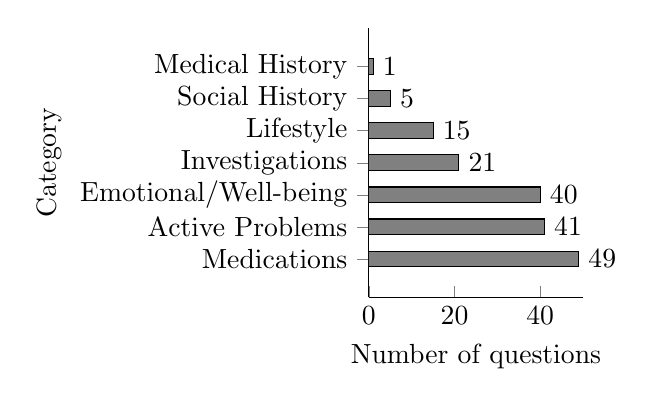
\begin{tikzpicture}
    \begin{axis}[
        xbar,
        width=4.3cm,
        height=5cm,
        bar width=0.2cm,
        nodes near coords,
        nodes near coords align={horizontal},
        xlabel={Number of questions},
        ylabel={Category},
        symbolic y coords={Medications, Active Problems, Emotional/Well-being, Investigations, Lifestyle, Social History, Medical History},
        ytick=data,
        xmin=0,
        xmax=50,
        enlarge y limits=0.2,
        axis x line*=bottom,
        axis y line*=left,
        ]
        \addplot [fill=gray, draw=black] coordinates {
            (49,Medications)
            (5,Social History)
            (41,Active Problems)
            (21,Investigations)
            (40,Emotional/Well-being)
            (15,Lifestyle)
            (1,Medical History)
        };
        % \draw[blue,dashed] ({axis cs:18.92,0}|-{rel axis cs:0,0}) -- ({axis cs:18.92,0}|-{rel axis cs:0,1}) node [pos=0.9, right] {STD = 18.92\%};
        % \draw[red,solid] ({axis cs:24.57,0}|-{rel axis cs:0,0}) -- ({axis cs:24.57,0}|-{rel axis cs:0,1}) node [pos=0.7, right] {Avg (24.57\%)};
    \end{axis}
\end{tikzpicture}
\caption{Number of questions asked in each category during the mock SRMs.}
\label{fig:question-categories}
\end{figure}

Of the four mock SMRs, a total of 117 questions were extracted from the transcripts generated by Microsoft Teams recordings. The questions were first extracted using OpenAI ChatGPT4 \cite{openai2023chatgpt4} to analyse the transcripts using this prompt "these are mock patient-doctor consultations, extract all the questions asked by the doctors". This was followed by manually checking each of the 117 questions within the video recordings to avoid transcription and extraction errors. The list of questions can be found in the first supplementary document. The questions were then grouped into these categories: conditions, medications, investigations, emotional/well-being, lifestyle, personal, and personal histories.

These categories were later presented to two of our clinician co-authors for an expert review. They made some changes in the categorisation with the final categories being \textit{active problems}, medications, investigations, emotional/well-being, lifestyle, \textit{social history} and \textit{medication history}. For the remainder of this work, we will refer to active problems as "conditions". This was followed by a review of question categorisation (which question belongs to which category on a spreadsheet) by the clinicians. The final categorisation of the questions is summarised in Figure \ref{fig:question-categories}, which shows that the highest number is 49 in the category of medications. The medical history category has the least number of questions. The top four categories by number of questions are conditions, medications, investigations, and emotional/well-being. The present work will focus on the following three categories of questions: \textbf{conditions}, \textbf{medications} and \textbf{investigations}. The number of questions in combinations of these three categories is listed in Table \ref{table:q-combination-stats}. 
\begin{table}[h]
\captionsetup{justification=justified}
\caption{The table shows the number of mock SMR questions about conditions, medications and investigations.}
\centering            % centres the whole table on the page
\begin{tabular}{>{\raggedright\arraybackslash}p{4.2cm} c}
\toprule
Combination & Question Count \\
\midrule
Medications &  35 \\
Conditions &  17 \\
Conditions, Medications &  13 \\
Conditions, Investigations &  10 \\
Investigations &  10 \\
Conditions, Medications, Investigations &   1 \\
\bottomrule
\end{tabular}
\label{table:q-combination-stats}
\end{table}

% \subsubsection{Time}
% The average time for an SMR was approximately 13 minutes (standard deviation: 4.24), and the time spent on the four main EMIS tabs is shown in Table \ref{table:smr-data-summary}. The average time spent by clinicians looking at problems, medications, investigations, and consultations was 1.65, 8.63, 3.23 and 0.47 minutes, respectively.The medication tab has the highest average, which is expected as the main aim of SMRs is a medication review. 

% ** Understanding the questions**
\subsection{Data abstraction} \label{sec:design-requirements}

\begin{table*}[ht]
\centering
\caption{The table shows breaking down questions asked during mock SMRs to generic data attributes required for each category of questions. The present work considers "dose" to be a quantitative value.}
\begin{tabularx}{\linewidth}{|X|>{\raggedright}m{2cm}|>{\raggedright\arraybackslash}m{2cm}|}
\hline
\textbf{Question} & \textbf{Data Attributes} & \textbf{Question Category} \\
\hline
What about taking the medicines because you're on quite a few. How do you feel about those?  & \multirow{3}{*}{Name} & Medications \\
Has anybody ever mentioned something called COPD to you? & & Conditions \\ 
Did he end up getting a scan in the end or not? & & Investigations \\ \hline
Have you been on the two for a long time?  & \multirow{3}{*}{Name, Date} & Medications\\ 
Have you had a recent blood test looking for hepatitis? &  & Investigations \\ 
Did that [diabetes] start later on? & & Conditions \\ \hline
I see that you're being put on some fairly strong painkillers. You don't feel very strong, no?  & Name, Dose & Medications \\ \hline
Have you ever had any specialist pain advice? & Name, Date, Severity & Conditions \\ \hline
Is that[diabetes] controlled at the moment?  & Name, Date, Quantity & Investigations \\ \hline
Here's your blood pressure?  & Quantity & Investigations \\ \hline
\end{tabularx}

\label{table:questions-to-data-attributes}
\end{table*}

Having looked at the content and duration of the SMRs, the questions were further analysed to determine the data required for each category: \textbf{conditions}, \textbf{medications} and \textbf{investigations}. The first step was to list what pieces of information are required by clinicians to answer each question within those categories (for details, see the supplemnetary material). From this list, for each of the questions, the combination of information such as name only, name and date, or a combination of name, date and other details was extracted. We call this information data attributes. For instance, for the question "Have you been on the two for a long time?" the required data was recorded as "medications" and "dates". 

The next step was to identify the data types of the information required by each question. For example, names (of conditions or medications) being "nominal". The data types used are nominal, quantitative, temporal, and ordinal. These are based on the taxonomy by Elshehaly et. al. \cite{elshehal2018taxonomy} which is based on the Vega \cite{satyanarayan2015reactive} data types. 

% There is work \cite{starren2000object} that categorises medical records into three data types: nominal, quantitative, and ordinal. 

The final step was to group the questions into possible combinations of data attributes for each category of question. The final output of this data abstraction process is summarised in Table \ref{table:questions-to-data-attributes}.

\subsection{Summary}

Four mock SMRs were performed to understand and characterise the domain problem (SMRs) believed to be the first of its kind for the purpose of a visualization design study focused on patient history visualization. The transcipts of these mock SMRs were analysed and a list of questions was extracted.  From these questions a data abstraction was generated that scoped the design study, which will be discussed next.

